	\section{Air Pollution}\label{sec:introdairpollution}
Air pollutants are particulates or gases in the air that harm human health or the economy and are present in concentrations that are unusual compared to background levels.  They can be created as a direct result of human actions (e.g. coarse particulates from construction or wood burning), as a secondary result created by chemical or physical processes in the atmosphere (e.g. ozone or nitrous oxides), or as a result of a natural process (e.g. forest fires or dust storms).  The \ac{EPA} has defined six \glspl{crit_pol} to be monitored that provide a good overview of air quality.  One of these is \ac{PM10}, the focus of this report,  with criteria set out in the US EPA NAAQS table.
%\citep{EPA:NAAQS_table})

\subsection{Air Pollution Monitoring: a History}
\label{sec:apmonitoring}
Air pollution has been monitored by national government agencies since the 1950s.  The most common motivation is the regulation of polluting industries and the preservation of population health, but other concerns include damage to buildings and infrastructure, reduced crop yields, and reduced air visibility.  

In the United Kingdom, the 1956 Clean Air Act was passed in response to high concentrations of Black Smoke (mostly particulates from coal burning) that, in 1952, was associated with 4000 excess deaths \cite{shaddick2014case}.

In the USA, the \ac{CAA} of 1963 created a regulatory system requiring states to work towards target goals for a range of air pollutants.  The Air Quality Act of 1967 created federal powers to monitor and enforce standards of air pollution, and in 1970 the creation of the \ac{EPA} consolidated these powers in a single agency %\citep{EPA:history}
.  The act was amended in 1977 and again in 1990 to reflect a changing understanding of pollutant creation and impact.  

The Los Angeles basin in particular has a long history of poor air quality.  Efforts to regulate and monitor air quality started in 1947 with the founding of the Los Angeles County Air Pollution Control District in response to widespread smog in 1943 
%\citep{CARB:History}
.



\section{Monitoring Air Pollution fields} \label{sec:monitoring}
We now describe our study in more detail. It set out to detect the bias, described above, that might be present in the South California Air Basin monitoring region after several decades of data monitoring.  Southern California has a long history of air pollution dating to 1945 \citep{CASCAQMD:2015}.

Models that describe spatial fields generally assume a random placement of monitoring sites or an independence of the latent field underlying the pollution field.  However, the placement of monitoring sites is often not random. They are chosen to fulfill a range of constraints and even if the initial selection is well-designed, sites might be chosen for termination because they are consistently in compliance.  This selection bias, referred to as \ac{PS}, can result in models that don't reflect the pollution field experienced by the population. 

Concern about \ac{PS} has a decade's long history. \citet{isaaks1988spatial} discuss how clustered data make variograms poor at estimating covariance parameters. \cite{diggle:07} define \ac{PS} in their book as the stochastic dependence of site locations upon the property being measured. \cite{shaddick2012preferential} discovered  \ac{PS} in the United Kingdom's black smoke monitoring network. Numerous other papers have examined \ac{PS} in different cases, showing how the \ac{PS} results in models incorrectly attributing the magnitude of pollution with impact on health or other model parameters.  An extensive list of references can be found in \citep{Zidek:2012}.  

The data gathered in the USA is freely available to the public and so gets put to many different uses.  Government agencies use this data to make real-time air quality warnings, to monitor general compliance of regions to meet predefined standards and to monitor point sources.  Healthcare specialists use the data from the monitoring in correlational studies to predict the health impacts of pollutant levels on the general population and subsets of interest.  \cite{wong2004comparison} brought up various concerns about using different interpolation techniques with \ac{EPA} data for epidemiological studies.  This combination of circumstances led us to be curious about whether the monitoring networks of the US exhibit \ac{PS}.


%\subsection{PM10 Pollution}
subsection{PM10 Pollution}
\label{sec:pm10}
Because the \ac{EPA} warehouses data on all the monitored pollutants, there is a choice of hundreds of pollutants, several of which could be reasonably chosen for analysis.  \ac{PM25} is currently considered more relevant for human health.  Ozone is a primary concern in LA because it is out of compliance.   Our study focussed on \ac{PM10} as follow-through on black smoke work in England by \cite{zidek2010monitoring}.  As well, \ac{PM10} has a longer history of monitoring in the \ac{SOCAB} than does \ac{PM25}.

\subsubsection*{What is PM10?}
\label{subsubsec:pm10nature}
\ac{PM10} are particulates with a diameter less than 10 $\mu m$ in diameter.  It is reported as a mass of solids per volume of air.  The coarser ($> 2.5 \mu m$ diameter) particles are generally a product of physical wear and tear, while the finer ($< 2.5 \mu m$ diameter) particles are usually aggregates from chemical reactions producing nitrogen and sulphur oxides
%\citep{EPA:PM_basics}
.

\subsubsection*{Effects of PM10}
\label{subsubsec:pm10effects}
These particulates have various deleterious effects on human health and infrastructure.  Health effects include both short and long-term concerns.  Short-term, high concentrations of \ac{PM10} can result in acute respiratory problems.  Long-term exposure to lower pollution levels can result in a chronic reduction in functionality of the lungs and cardiovascular system %\citep{EPA:PM_impact}
.  Economically \ac{PM10} damages property, crops, and reduces visibility
%\citep{EPA:PM_impact}
.

\subsubsection*{Measurement of PM10}
\label{subsubsec:pm10measurement}
Measuring a field that is continuous in time and space can be challenging.  Typically, discrete measurements are taken, and a model interpolates these to estimate a field.  As a result, these measurements are interpreted as averaging over both a spatial and temporal range.

Spatial averaging at each site represents a mass of upwind air, its volume depending upon the geography of each site and the pollutant being monitored.  This is acknowledged in the spatial scale provided in the reports.   

In Appendix D Section 4.6 (b) of CFR 40-58 %\ac{PM10} sensors are said to monitor air on a scale of $100 m$ to $ 4~km $ depending upon the homogeneity of the air and surface \citep{CFR:Title40-58}.


Temporal averaging of the observations is a property of the measurement technique.  The US's gold standard for \ac{PM10}, the \ac{FRM}, is to pull air through filters and weigh the accumulated particles after 24 hours.  This gives an average particulate presence in the air over 24 hours.  The frequency at which these 24-hour samples are taken depends upon the pollutant levels, with levels closer to the standards requiring more frequent measurements (see table \ref{tab:EPA_monitoring_freq}) 
\citep{CASCAQMD:2015}.

Other measurement techniques are called \ac{FEM}.  Laser back-scatter measurements provide instantaneous readings of particulate size and concentration, generally taken every few minutes.  These are useful for delivering time-sensitive warnings.  In the yearly reports, these \ac {FEM} are averaged over 24hrs to be temporally equivalent to the \ac{FRM} instrumentation.

Individual sites often have multiple instruments monitoring the same pollutant. For example, there could be a continuous \ac{FEM} monitor for forecasting as well as air quality advisories and one \ac{FRM} monitor to fulfill statutory requirements.  Other reasons to have multiple monitors include research or sensor calibration. 



\subsection{Government Administration}
\label{subsec:govtadmin}
The process of interest-choice of site location and the possible subsequent preferential sampling is a product of governmental decisions to set and meet regulatory standards.  For the United States, these regulations are described in detail on the EPA website
%\ac{EPA} website 
but outlined here.
%\citep{EPA:PM10_NAAQS}.

\subsubsection*{Regulatory Framework in the US}
\label{subsubsec:regulation}
In the United States, air quality monitoring and enforcement requires cooperation and coordination between governmental agencies at the regional, state and federal levels.

At the Federal level, the \ac{EPA} defines standards for air quality levels, monitoring and reporting.   These standards define:
\begin{enumerate}
	\item the levels of pollution that must not be exceeded;
	\item how to monitor each pollutant (number and location of sites, frequency of monitoring, and what methods count as \ac{FRM});
	\item when and how to make reports to the \ac{EPA}.
\end{enumerate}

The states divide themselves into regional districts responsible for choosing site placement and report preparation.  States can set their regulations, but must still meet the \ac{EPA}'s regulations. 

\subsubsection*{Air Quality Standards}\label{subsubsec:aqs}
The \ac{CAA} established six important pollutants, called \gls{crit_pol}, 
including particulate matter, and gave the \ac{EPA} power to define \acp{NAAQS} for each.

The \ac{EPA} sets two standards to meet health and economic goals, known respectively as the primary and secondary standards.  Primary standards:
\begin{quote}
	``Provide public health protection, including protecting the health of `sensitive' populations such as asthmatics, children, and the elderly.'' 
\end{quote}
Secondary standards:
\begin{quote}
	``Provide public welfare protection, including protection against decreased visibility and damage to animals, crops, vegetation, and buildings.''  
\end{quote}
These criteria can be 
seen in the US EPA NAAQS table
at the URL\\
www.epa.gov/pm-pollution \\/timeline-particulate-matter-pm-national-ambient-air-quality-standards-naaqs\#Superscript1

In 2006, the EPA revoked the primary annual \ac{NAAQS} for \ac{PM10} meaning that \ac{PM10} is no longer seen as problematic long term.  Short-term \ac{PM10} pollution remains a concern and is monitored for 24-hour primary exceedance in the US 
%\citep{EPA:PM10_NAAQS}
.  Table \ref{tab:EPA_PM10_standards} shows how the averaging time and core statistic have changed historically, and how the acceptable concentration has decreased since the initial creation of the \ac{PM10} \ac{NAAQS} in 1971 
%\citep{EPA:PM10_NAAQS}
.
\begin{table}[ht]
	\centering
	\begin{tabular}{p{0.06\textwidth}|p{0.18\textwidth}|p{0.15\textwidth}|p{0.14%\textwidth}|p{0.36
				\textwidth}|p{0.30
				\textwidth}}
		Year & Final Rule / Date & Averaging Time & Level & Form \\
		\hline
		1997 & 62 FR 38652 Jul 18, 1997, & 24 hour & 150 $\mu g/m^3$ &	Initially promulgated 99th percentiles, averaged over 3 years; when 1997 standards for PM10 were vacated, the form of 1987 standards remained in place (not to be exceeded more than once per year on average over 3 years) \\
		1997 & 62 FR 38652 Jul 18, 1997 & Annual & 50 $\mu g/m^3$ & Annual arithmetic mean, averaged over 3 years \\
		2006 & 71 FR 61144 Oct 17, 2006, & 24 hours & 150 $\mu g/m^3$ & Not to be exceeded more than once per year on average over 3 years \\
		2012 & 78 FR 3085 Jan 15, 2013 & 24 hour & 150 $\mu g/m^3$ & Not to be exceeded more than once per year on average over 3 years \\
	\end{tabular}
	\caption{Abridged history of Primary and Secondary standards for PM10.  The \ac{EPA} revoked the annual PM10 \ac{NAAQS} in 2006, but maintains the acute 24hr standard 
	}
	\label{tab:EPA_PM10_standards}
\end{table}

In addition to these federal standards, California has its own set of standards that are more stringent (24-hour: $50 \mu g/m^3$, Annual: $20 \mu g/m^3$).  However, these are not considered for this report since it focuses on \ac{EPA} standards and monitoring.

\subsubsection*{Monitoring Requirements}\label{subsubsec:monreqs}
The requirements to design and set up a monitoring network are proscribed in the \ac{CFR}, Title 40, Subsection 58 appendix D \citep{CFR:Title40-58}.

The minimum number of sensors for a given region is based upon both the population and the concentration of \ac{PM10} relative to It's \ac{NAAQS} as described in table \ref{tab:NAAQS_site_count}.
\begin{table}[ht]
	\centering
	\begin{tabular}{p{0.25\textwidth}|p{0.18\textwidth}|p{0.18\textwidth}|p{0.18\textwidth}}
		Population category of \ac{MSA} & High (PM10 > \ac{NAAQS} * 1.2) & Medium (PM10 > \ac{NAAQS} *0.8) & Low (PM10 < \ac{NAAQS}*0.8) \\
		\hline
		> 1,000,000 & 6-10 & 4-8 & 2-4 \\
		500,000 - 1,000,00 & 4-8 & 2-4 & 1-2 \\
		250,000 - 500,000 & 3-4 & 1-2 & 0-1 \\
		100,000 - 250,000 & 1-2 & 0-1 & 0 \\
	\end{tabular}
	\caption{How the required number of sites for monitoring PM10 increases with both the population of the Metropolitan Statistical Area and the severity of the ambient pollution \citep{CFR:Title40-58}. }
	\label{tab:NAAQS_site_count}
\end{table}

The monitoring frequency is dependent upon the site's pollution concentration relative to that pollutant's standard, as described in table \ref{tab:EPA_monitoring_freq}  \citep{AQMNP:2019}.

\begin{table}[ht]
	\centering
	\begin{tabular}{p{0.25\textwidth}|p{0.10\textwidth}|p{0.13\textwidth}|p{0.13\textwidth}|p{0.13\textwidth}|p{0.08\textwidth}}
		Ratio of previous Pollutant level to standard & $<0.8$ & $(0.8 < 0.9)$ & $(0.9 < 1.2)$ & $(1.2 < 1.4)$ & $1.4<$  \\
		\hline
		Monitoring frequency & Every 6th day & Every other day & Every Day & Every other day & Every 6th day \\ 
	\end{tabular}
	\caption{How the monitoring frequency of a given site depends upon how close it is to the \ac{NAAQS} exceedance threshold \citep{AQMNP:2019}.}
	\label{tab:EPA_monitoring_freq}
\end{table}

\subsubsection*{Spatial Scale}
\label{subsubsec:spatscale}
Each site has a spatial scale defined in Appendix D Section 1.2 of \ac{CFR} 40. The purpose of defining the spatial scale:
\begin{quote}
	``Is to correctly match the spatial scale represented by the sample of monitored air with the spatial scale most appropriate for the monitoring site type, air pollutant to be measured, and the monitoring objective.''  \cite{CFR:Title40-58}
\end{quote}
Sites monitoring \ac{PM10} generally have two relevant scales, the Middle scale ($100~m - 500~m$) and the Neighborhood scale ($0.5~km - 4.0~km$).  

\subsubsection*{Monitoring Purpose}
\label{subsubsec:purpose}
Each site has at least one monitoring purpose, which: 
\begin{quote}
	``Is the reason why a certain pollutant is being measured at a certain site.'' \citep{AQMNP:2019} 
\end{quote} The full list of all purposes 
is quite lengthy
%and their definitions are in the Appendix,
but there are only two purposes relevant for sites monitoring \ac{PM10} in the \ac{SOCAB}.  
\begin{itemize}
	\item \textbf{High concentration} monitoring is conducted at sites to determine the highest concentration of an air pollutant in an area within the monitoring network. A monitoring network may have multiple high-concentration sites (i.e., due to varying meteorology year to year).
	\item \textbf{Population exposure} monitoring is conducted to represent the air pollutant concentrations to which that populated area exposed 
	\citep{AQMNP:2019}.
\end{itemize}


\subsubsection*{Reporting Requirements}
\label{subsubsec:ReportingRequirements}
Reporting air quality data is mandated by the \ac{EPA}.  Each year, regional monitoring districts compile the past year's data and submit it to the \ac{EPA} for entry into a publicly accessible database.  After data cleaning, the \ac{EPA} makes the reported data available as recompiled data files on its website at \url{https://aqs.epa.gov/aqsweb/airdata/download_files.html}.  

The \ac{AQMP} is a report written every 3–4 years by the local \ac{AQMD} that summarizes whether the region is in or out of attainment of the Federal levels for all \glspl{crit_pol}.
Every 5 years, a full site visit and Network Assessment is done to produce a report on the state of the network. These reports for the \ac{SCAQMD} were done in 2010 and 2015.  Each report describes the sites in the network, including the site's Monitoring Purpose and Spatial Scale.  While most regions in California prepare their reports through the California Air Resources Board, the \ac{SCAQMD} prepares and submits its report separately.



\subsection{The LA Basin} \label{subsec:labasin}
A \gls{air_basin} is a geographic region of roughly similar air conditions, typically a topographic depression.  The \ac{SOCAB} is approximately 17 to 100 square kilometres \gls{air_basin} surrounding Los Angeles.  It can be seen depicted in Figure \ref{fig:SOCAB_counties}.  Its boundary is different from the jurisdiction of the body that manages the \gls{air_basin}, the \ac{SCAQMD}. The \ac{SCAQMD}, in Figure \ref{fig:SCAQMD-jurisdiction} consists of four counties and exists over several \glspl{air_basin}.  


The \ac{SOCAB} is defined in the California Code of Regulations Title 17  Subchapter 1.5  Article 1.  § 60104.   
\begin{quote}
	``South Coast Air Basin means the non-desert portions of Los Angeles, Riverside, and San Bernardino counties and all of Orange County as defined in California Code of Regulations, Title 17, Section 60104. The area is bounded: on the west by the Pacific Ocean; on the northwest by the Santa Susana Mountains and Simi Hills, on the north by the San Gabriel Mountains, San Bernardino Mountains, and on the east by the San Jacinto Mountains and Santa Rosa Mountains; and on the south by the San Diego County line.''
	
\end{quote}
%https://ww3.arb.ca.gov/regs/title17/60104.pdf

\begin{landscape}
	\begin{figure}[ht]
		\captionsetup{justification=centering}
		\caption{This map made by the \ac{AQMD} shows how the jurisdiction and the air basin overlap.\\  The main figure shows the \ac{SCAQMD} and the insert in the top right corner demonstrates \\where the \ac{SOCAB} is in relation to the \ac{SCAQMD}. All the \ac{SOCAB} lie in the \ac{SCAQMD}.\\ But the \ac{SCAQMD} stretches over parts of several airsheds.  
		}
		\centering
		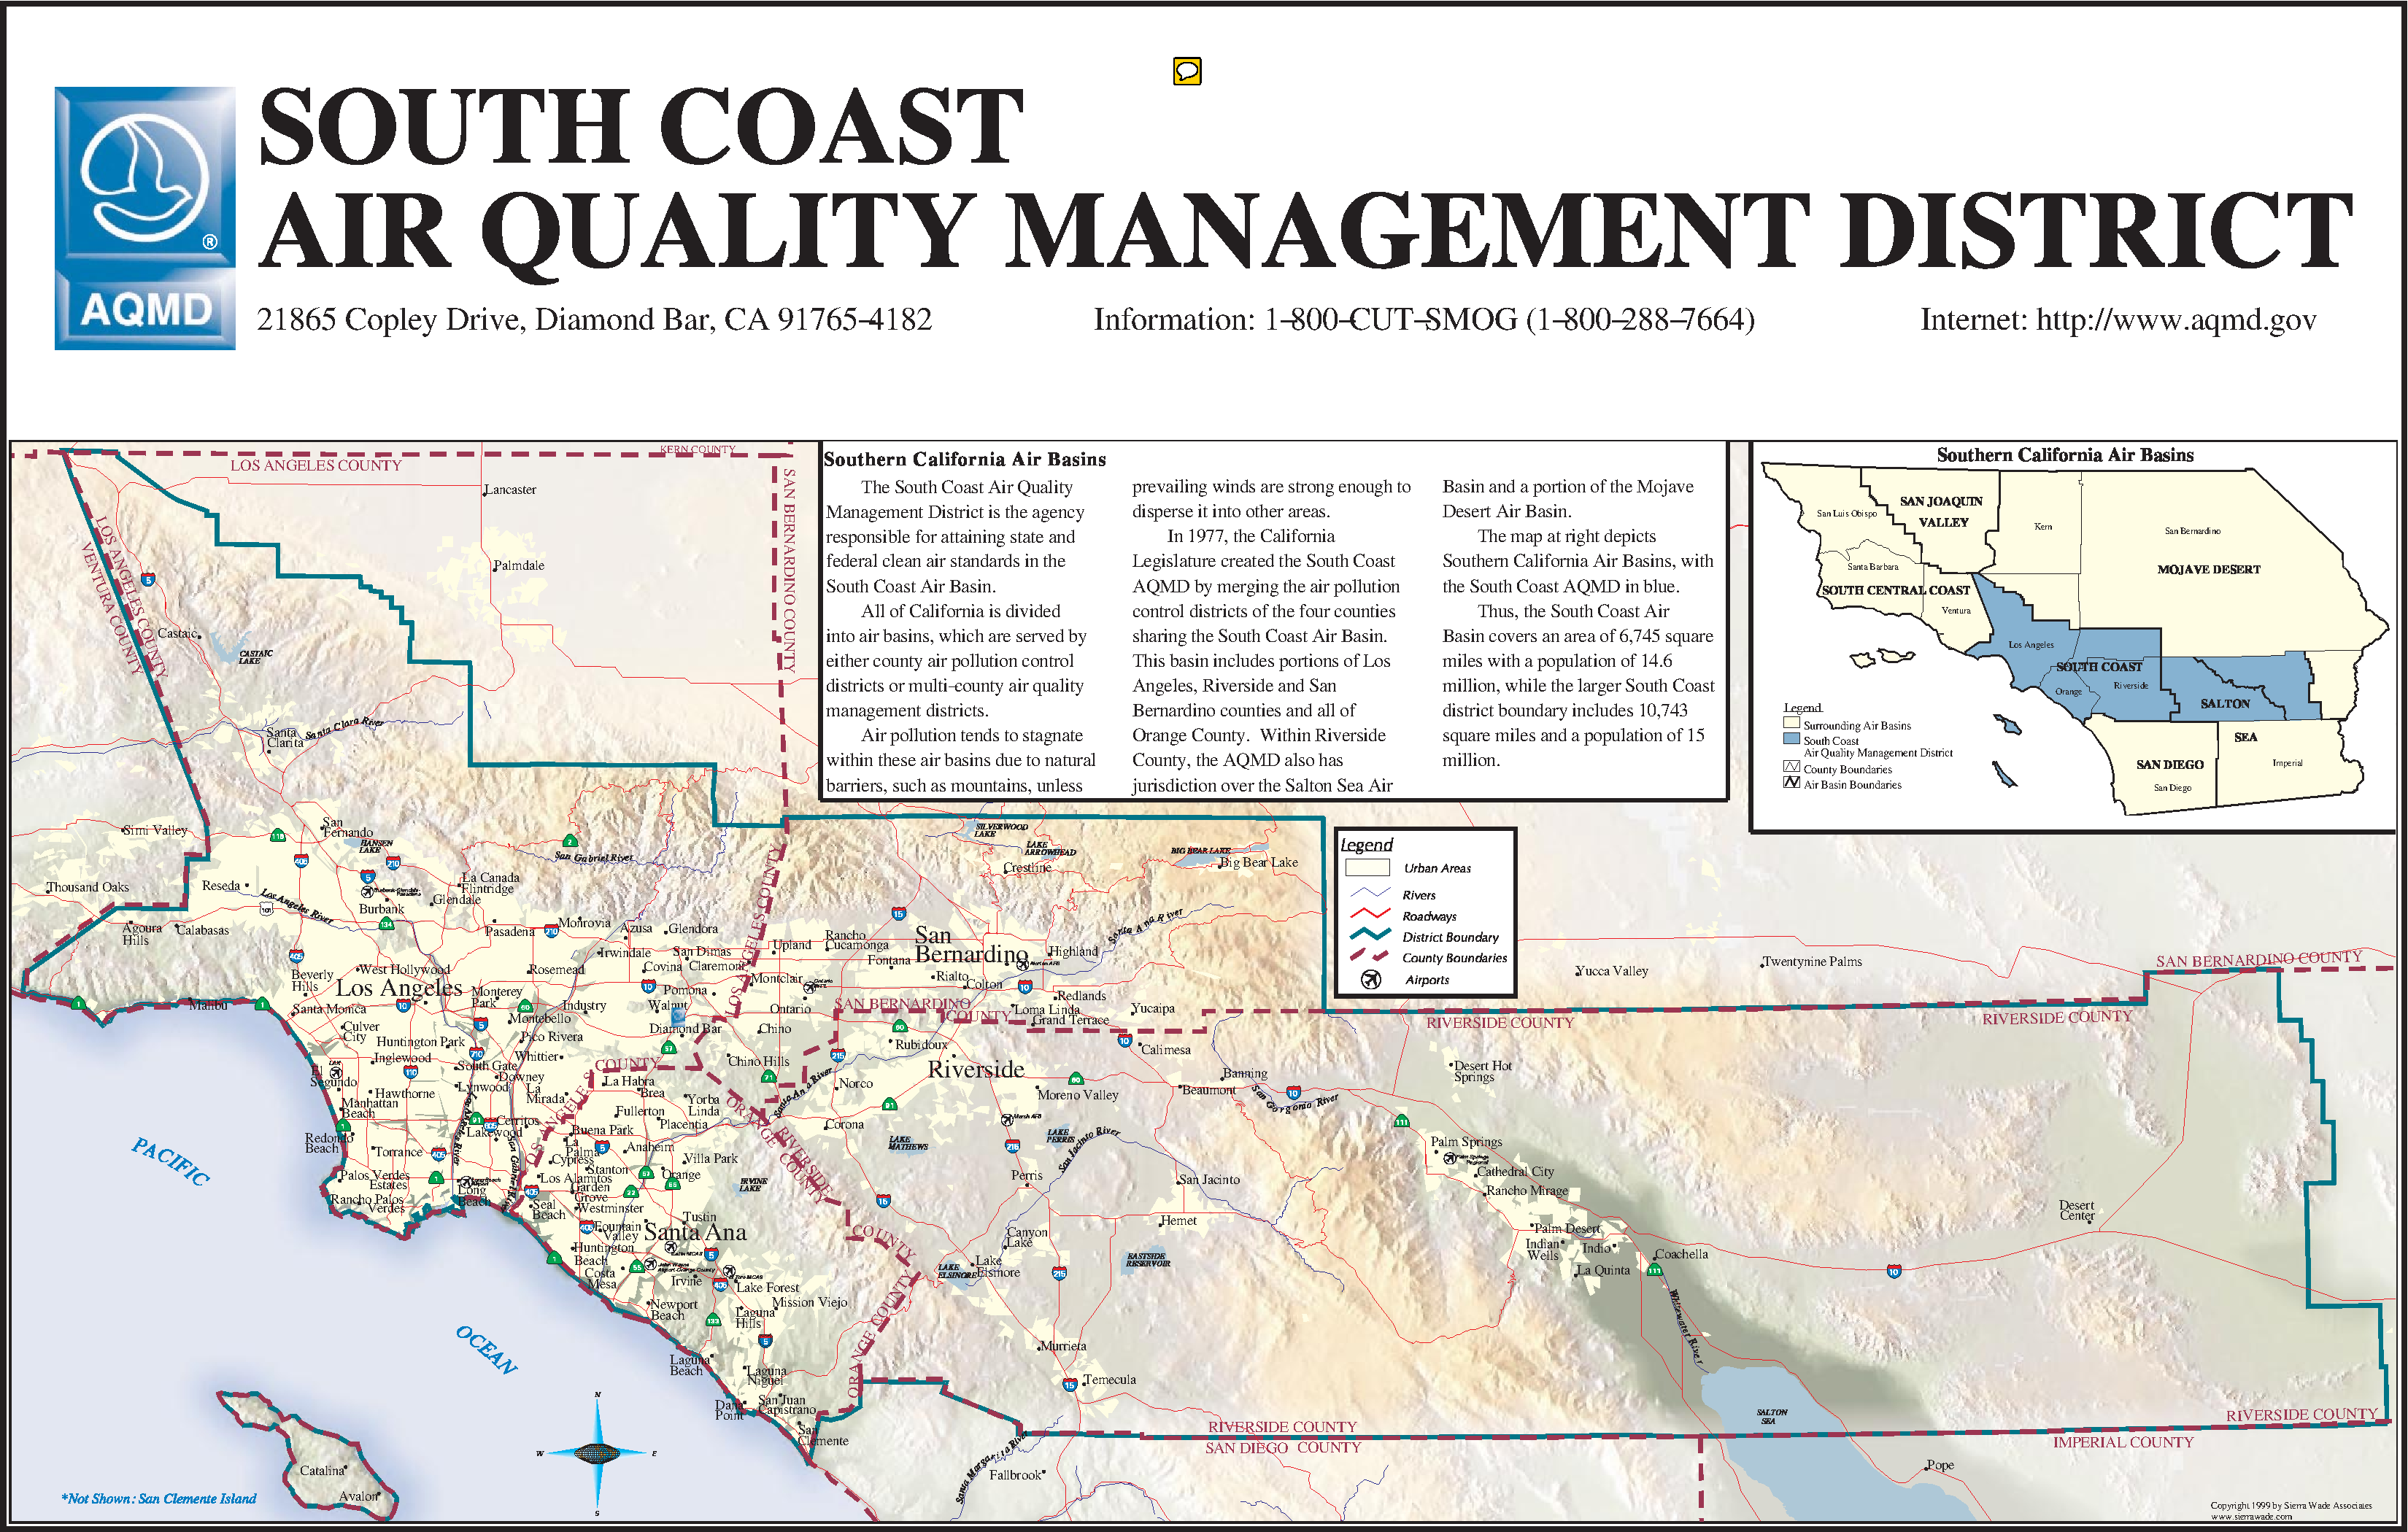
\includegraphics[width = \textwidth]{Figures/map-of-jurisdiction.pdf}
		\label{fig:SCAQMD-jurisdiction}
	\end{figure}
\end{landscape}


%History of attainment for the SOCAB: %https://ww2.arb.ca.gov/our-work/programs/state-and-federal-area-designations/state-area-designations/summary-tables
%Map comparing regions in Cali based upon Cali reqs and Federal reqs.
%https://ww2.arb.ca.gov/resources/documents/maps-state-and-federal-area-designations
%Population?
%Pollution history
%CUrrent regional trends: %https://www.epa.gov/air-trends/particulate-matter-pm10-trends  %Described regional trends